\section{Árvores de regressão}\label{sec:regressao}

\begin{frame}{Da classificação à regressão: o que muda?}
\begin{itemize}
  \item A resposta agora é \alert{numérica}. A árvore continua sendo uma partição do espaço em retângulos $p$-dimensionais.
  \item Em cada folha, a previsão deixa de ser uma \alert{classe} (a moda) e passa a ser um \alert{número}: a \alert{média} das respostas das observações que caíram ali.
  \item O erro deixa de contar acertos e passa a medir a \alert{distância} entre $y_i$ e a previsão: a impureza do nó é a \alert{variância}.
  \item Tudo o mais é reaproveitado: perguntas $x_j\le\tau$, busca gulosa, condição de parada, poda.
\end{itemize}
\vspace{4pt}
\begin{block}{Exemplo corrente: \emph{diabetes} (scikit-learn)}
$442$ pacientes. Resposta: \alert{progressão da doença} um ano após a coleta (índice numérico). Preditores: idade, sexo, IMC, pressão e $6$ medidas de sangue. Começamos só com o \alert{IMC}, para poder \alert{desenhar} o ajuste.
\end{block}
\end{frame}

\begin{frame}[fragile]{API do scikit-learn: \texttt{DecisionTreeRegressor}}
\begin{lstlisting}[style=py]
DecisionTreeRegressor(*, criterion='squared_error', splitter='best',
    max_depth=None, min_samples_split=2, min_samples_leaf=1,
    max_features=None, random_state=None, max_leaf_nodes=None,
    min_impurity_decrease=0.0, ccp_alpha=0.0, ...)
\end{lstlisting}
\vspace{2pt}
\footnotesize
\begin{tabular}{@{}p{0.26\linewidth}p{0.68\linewidth}@{}}
\toprule
\texttt{criterion} & \texttt{'squared\_error'}: variância (nosso $\mathrm{RSS}$); também \texttt{'absolute\_error'} (mediana) e \texttt{'poisson'}\\
\texttt{max\_depth} & profundidade máxima $h_{\max}$ (\texttt{None}: sem limite)\\
\texttt{min\_samples\_leaf} & mínimo de observações por folha\\
\texttt{ccp\_alpha} & $\alpha$ da poda por custo-complexidade\\
\midrule
métodos & \texttt{fit}, \texttt{predict}, \texttt{score} (devolve $R^2$)\\
atributos & \texttt{tree\_}, \texttt{get\_n\_leaves()}, \texttt{feature\_importances\_}\\
\bottomrule
\end{tabular}

\vspace{2pt}
{\scriptsize Compare com \texttt{DecisionTreeClassifier}: muda o \texttt{criterion} (\texttt{'gini'}, \texttt{'entropy'}).}
\end{frame}

\begin{frame}[fragile]{Exemplo em Python: uma árvore de profundidade 2}
\lstinputlisting[style=py]{../python/regressao/01_arvore_bmi.py}
\vspace{4pt}
\begin{itemize}
  \item \texttt{export\_text} imprime as regras da árvore ajustada (próximo slide).
  \item O RMSE é a raiz do erro quadrático médio no teste, na unidade de $y$.
\end{itemize}
\end{frame}

\begin{frame}[fragile]{Lendo o resultado}
\begin{columns}[T]
\column{0.46\textwidth}
\lstinputlisting[style=saida,basicstyle=\ttfamily\fontsize{7}{8.4}\selectfont]{../python/regressao/outputs/01_arvore_bmi.txt}
\column{0.52\textwidth}
\small
\begin{itemize}
  \item Quatro folhas, quatro previsões: $106{,}9$, $138{,}2$, $190{,}0$ e $271{,}1$. Cada uma é a \alert{média} de $y$ no treino na sua região do IMC.
  \item Primeiro corte em $\text{IMC}\le0{,}01$; depois em $-0{,}02$ e $0{,}07$: o algoritmo escolheu \alert{onde} cortar para minimizar o RSS.
  \item RMSE no teste $=62{,}7$ contra desvio-padrão de $y$ de $74{,}7$: a árvore explica \alert{pouco}, esperado com uma só variável.
  \item Duas perguntas: \alert{por que} esses cortes (metodologia e algoritmo)? \alert{Quantas} folhas usar (sobreajuste)?
\end{itemize}
\end{columns}
\end{frame}

\begin{frame}{Metodologia $\times$ algoritmo}
\begin{columns}[T]
\column{0.485\textwidth}
\begin{block}{Metodologia: \emph{o que queremos}}
\small
Um \alert{modelo} e um \alert{critério}:
\begin{itemize}
  \item modelo: $\hat f(\mathbf x)=\sum_{m=1}^M \bar y_m\,\ind(\mathbf x\in R_m)$, com $R_1,\dots,R_M$ retângulos disjuntos;
  \item critério: escolher $R_1,\dots,R_M$ que minimizam
  \[\mathrm{RSS}=\sum_m\sum_{\mathbf x_i\in R_m}(y_i-\bar y_m)^2 .\]
\end{itemize}
É um \alert{problema de otimização}. Não diz como resolvê-lo.
\end{block}
\column{0.485\textwidth}
\begin{block}{Algoritmo: \emph{como obtemos}}
\small
Uma \alert{receita} que aproxima a solução:
\begin{itemize}
  \item testar \alert{todas} as partições é inviável (cresce explosivamente com $n$ e $p$);
  \item então: busca \alert{gulosa}, de cima para baixo, em \alert{um corte por vez}: Alg.~\aGrow{} e \aBest;
  \item pare por $h_{\max}$, $n_{\min}$ ou nó puro; depois pode (Alg.~\aPrune).
\end{itemize}
Entrega uma árvore \alert{boa}, não necessariamente a de menor RSS.
\end{block}
\end{columns}
\vspace{4pt}
\centering\small
Mesma \alert{metodologia} $\Rightarrow$ algoritmos diferentes são possíveis (CART, ID3, C4.5, \dots). Mesmo \alert{algoritmo} $\Rightarrow$ metodologias diferentes (classificação e regressão).
\end{frame}

\begin{frame}{Metodologia: modelo e critério}
Resposta contínua. Em cada região, a previsão é a média:
\[
\hat f(\mathbf x)=\sum_{m=1}^M \bar y_m\,\ind(\mathbf x\in R_m),\qquad \bar y_m=\frac1{n_m}\sum_{\mathbf x_i\in R_m}y_i .
\]
O critério é a soma dos quadrados dos resíduos:
\[
\mathrm{RSS}=\sum_{m=1}^M\sum_{\mathbf x_i\in R_m}(y_i-\bar y_m)^2 .
\]
\begin{itemize}
  \item Por que a \alert{média}? Fixadas as regiões, $\bar y_m$ minimiza $\sum_{\mathbf x_i\in R_m}(y_i-c)^2$ em $c$: a média é a melhor constante.
  \item A impureza do nó é a \alert{variância}: $\Q_m=\dfrac1{n_m}\sum_{\mathbf x_i\in R_m}(y_i-\bar y_m)^2$.
\end{itemize}
{\footnotesize Morettin \& Singer (2021, \S10.4 e Nota de Capítulo~4).}
\end{frame}

\begin{frame}{Algoritmo: o mesmo, com outra impureza}
\begin{itemize}
  \item \textsc{CresceÁrvore} e \textsc{MelhorCorte} (Alg.~\aGrow{} e \aBest) valem sem mudanças, trocando $\Q$ por variância e $k(m)$ por $\bar y_m$.
  \item O melhor corte do nó minimiza $\mathrm{RSS}_L+\mathrm{RSS}_R$, equivalente a $\frac{n_L}{n_m}\Q_L+\frac{n_R}{n_m}\Q_R$.
  \item Varredura eficiente: manter $S_1=\sum y_i$ e $S_2=\sum y_i^2$ de cada lado; então
  \[
  \mathrm{RSS}_{\text{nó}}=S_2-\frac{S_1^2}{n_{\text{nó}}},
  \]
  e cada candidato custa $O(1)$.
  \item Poda por custo-complexidade: $R_\alpha(T)=\mathrm{RSS}(T)+\alpha|T|$, com o mesmo Algoritmo~\aPrune.
  \item Categóricas: níveis ordenados por $\bar y_c$ (teorema de Breiman, exato em regressão).
\end{itemize}
% [MANIM] corte candidato deslizando sobre o IMC e o RSS mudando
\end{frame}

\begin{frame}{A função em degraus, por profundidade}
\centering
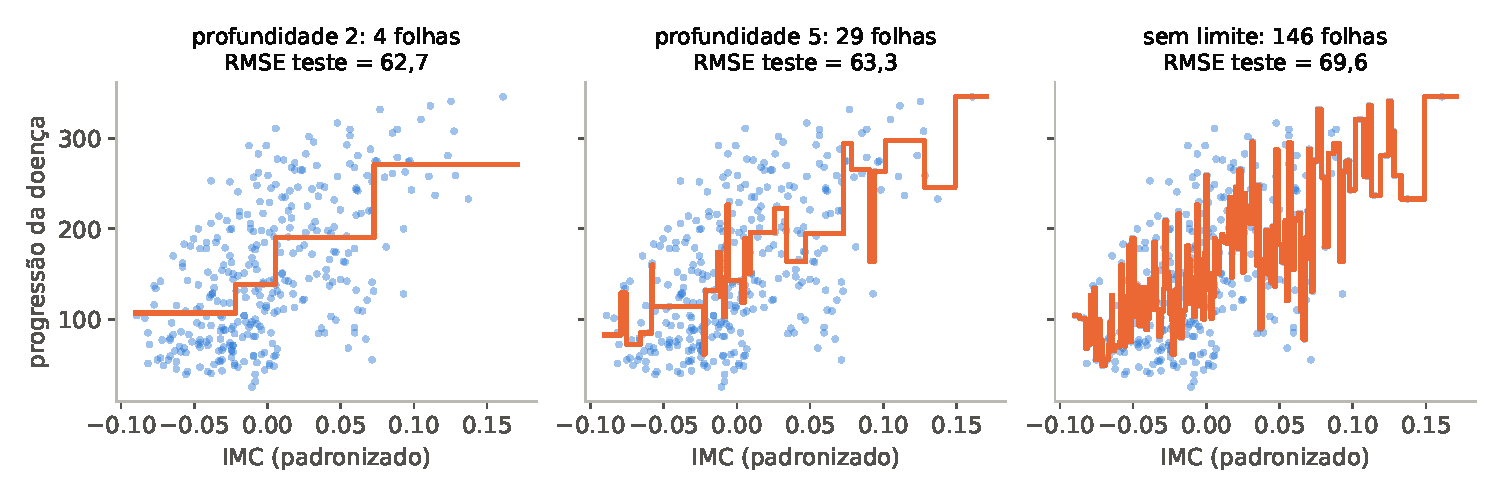
\includegraphics[width=\linewidth]{../python/regressao/figures/degraus.pdf}
\vspace{2pt}
\begin{itemize}
  \item Profundidade $2$: poucos degraus, curva grosseira (viés). Sem limite: $146$ folhas para $331$ pacientes de treino, \alert{decorando o ruído} (variância).
  \item O menor RMSE de teste está no meio. Próximo slide: em média de $30$ divisões.
\end{itemize}
% [MANIM] função em degraus aproximando os dados conforme a árvore cresce
\end{frame}

\begin{frame}[fragile]{Profundidade e sobreajuste em números}
\lstinputlisting[style=py,firstline=12,lastline=21]{../python/regressao/02_profundidade.py}
\vspace{3pt}
\lstinputlisting[style=saida]{../python/regressao/outputs/02_profundidade.txt}
\vspace{3pt}
{\small O RMSE de \alert{treino} só cai com a profundidade ($65{,}2\to47{,}0$); o de \alert{teste} cai até a profundidade $2$ ($64{,}3$) e sobe depois, chegando a $75{,}3$, perto do desvio-padrão de $y$.}
\end{frame}

\begin{frame}[fragile]{Escolhendo a complexidade por validação cruzada}
\lstinputlisting[style=py,firstline=9,lastline=16]{../python/regressao/03_validacao_cruzada.py}
\vspace{3pt}
\lstinputlisting[style=saida]{../python/regressao/outputs/03_validacao_cruzada.txt}
\vspace{3pt}
\begin{itemize}
  \item A validação cruzada ($5$ partes, só no treino) escolhe $h_{\max}=2$ e folhas com pelo menos $20$ pacientes.
  \item O RMSE no teste ($62{,}7$) fica próximo do estimado ($64{,}5$): a estimativa é honesta.
\end{itemize}
\end{frame}

\begin{frame}{Limitações das árvores de regressão}
\begin{block}{A função predita é descontínua e em degraus}
Não \alert{extrapola}: fora do intervalo do treino, devolve a média da folha de borda. Aproxima mal relações suaves ou lineares.
\end{block}
\begin{itemize}
  \item Uma única árvore é \alert{instável} (alta variância): $\Rightarrow$ bagging, florestas e boosting nas seções seguintes.
  \item No caso prático (Seção~\ref{sec:caso}), uma árvore completa tem RMSE \alert{pior} que uma reta com as $10$ variáveis.
\end{itemize}
\end{frame}
